\documentclass[UTF8]{ctexart}
% 基本设置和必要宏包
\usepackage{geometry}
\geometry{a4paper,scale=0.8}

% 数学相关宏包
\usepackage{amsmath}
\usepackage{amssymb}
\usepackage{amsfonts}

\usepackage{mathtools}
\usepackage{amsbsy}
\usepackage{amstext}
\usepackage{wasysym}
\usepackage{stmaryrd}
\usepackage{mathrsfs}

% 图形和颜色
%\usepackage{xcolor}
\usepackage{graphicx}
\usepackage{subcaption}
\usepackage{caption}
\usepackage{float}



% 其他功能性宏包
\usepackage{titlesec}
\usepackage{fancyhdr}
\usepackage{setspace}
\usepackage{cite}
\usepackage{appendix}
\usepackage{listings}
\usepackage{pdfpages}
\usepackage{enumitem}
\usepackage{tabu}
\usepackage{threeparttable}
\usepackage{booktabs}
\usepackage{abstract}


\usepackage{diagbox} 

\newcommand{\sihaoheiti}{\fontsize{14pt}\selectfont\heiti}
% 设置全局字体
%\setCJKmainfont{SimSun} % 设置正文为宋体
%\setCJKsansfont{SimHei} % 设置无衬线字体为黑体

% 论文题目设置为三号黑体字,并居中
\newcommand{\threelargebf}{\fontsize{16pt}{19.2pt}\selectfont\heiti\centering}

% 一级标题设置为四号黑体字,并居中
\titleformat{\section}{\centering\fontsize{14pt}{16pt}\bfseries\heiti}{\thesection}{1em}{}

% 二级标题设置为小四号黑体字,左对齐
\titleformat{\subsection}{\fontsize{12pt}{14.4pt}\bfseries\heiti}{\thesubsection}{1em}{\raggedright}

% 三级标题设置为小四号黑体字,左对齐
\titleformat{\subsubsection}{\fontsize{12pt}{14.4pt}\bfseries\heiti}{\thesubsubsection}{1em}{\raggedright}

% 正文字体设置为小四号宋体字,并使用单倍行距
\renewcommand{\normalsize}{\fontsize{12pt}{14.4pt}\selectfont}
%\renewcommand{\baselinestretch}{3}
%\selectfont



%\linespread{5.0}%修改行距
% 图片文件夹
\graphicspath{{img/}}
\let\itemize\compactitem
\let\enditemize\endcompactitem

% 设置页面布局
\geometry{a4paper, left=2.5cm, right=2.5cm, top=3cm, bottom=3cm}
\setstretch{1.5}

\renewcommand{\arraystretch}{1.5}
\newcommand{\thickhline}{\noalign{\hrule height 1.2pt}} % 设置粗线的宽度
\newcommand{\thinhline}{\noalign{\hrule height 0.8pt}} % 设置细线的宽度

%%%% ===== 定理环境
\usepackage[amsmath,thref,thmmarks,hyperref]{ntheorem} % 定理宏包
%\theorempreskipamount1em % spacing before the environment
%\theorempostskipamount0em  % spacing after the environment
%\theoremstyle{plain}
%\theoremheaderfont{\normalfont\heiti}
%\theorembodyfont{\normalfont\kaishu}
%\theoremindent0em
%\theoremseparator{\hspace{0.2em}}
%\theoremnumbering{arabic}

\newtheorem{property}{性质}[section]
\newtheorem{definition}{定义}[section]
\newtheorem{lemma}{引理}[section]
\newtheorem{remark}{注记}[section]
\newtheorem{corollary}{推论}[section]
\newtheorem{example}{例}[section] 
\newtheorem{problem}{{问题}}

 \renewcommand{\abstractnamefont}{\normalfont\bfseries}  % 摘要标题字体:正常字体,粗体
\renewcommand{\abstracttextfont}{\normalfont\normalsize}     % 摘要内容字体:正常字体,小四号

% 设置页眉页脚
\pagestyle{fancy}
\fancyhf{}
\fancyfoot[C]{\thepage}
\renewcommand{\headrulewidth}{0pt}

% 设置标题格式
\titleformat{\section}{\centering\heiti\large}{\thesection}{1em}{}
\titleformat{\subsection}{\raggedright\heiti\normalsize}{\thesubsection}{1em}{}
\titleformat{\subsubsection}{\raggedright\heiti\normalsize}{\thesubsubsection}{1em}{}

% 设置摘要环境
%\newenvironment{myabstract}{
%	\begin{center}
%	\bfseries\zihao{-3} 摘要
%	\end{center}
%	\vspace{-0.5em} % 调整摘要与论文题目的距离
%	\normalsize
%}{
%}
% 设置附录环境
\renewcommand{\appendixname}{附录}
\renewcommand{\appendixpagename}{附录}

% 设置代码环境
\lstset{
	basicstyle=\small\ttfamily,
	keywordstyle=\color{blue},
	commentstyle=\color{green!70!black},
	stringstyle=\color{red},
	breaklines=true,
	numbers=left,
	numberstyle=\tiny,
	frame=tb,
	language=Python
}
\newcommand{\bbA}{\mathbb{A}}
\newcommand{\bbB}{\mathbb{B}}
\newcommand{\bbC}{\mathbb{C}}
\newcommand{\bbD}{\mathbb{D}}
\newcommand{\bbE}{\mathbb{E}}
\newcommand{\bbF}{\mathbb{F}}
\newcommand{\bbG}{\mathbb{G}}
\newcommand{\bbH}{\mathbb{H}}
\newcommand{\bbI}{\mathbb{I}}
\newcommand{\bbJ}{\mathbb{J}}
\newcommand{\bbK}{\mathbb{K}}
\newcommand{\bbL}{\mathbb{L}}
\newcommand{\bbM}{\mathbb{M}}
\newcommand{\bbN}{\mathbb{N}}
\newcommand{\bbO}{\mathbb{O}}
\newcommand{\bbP}{\mathbb{P}}
\newcommand{\bbQ}{\mathbb{Q}}
\newcommand{\bbR}{\mathbb{R}}
\newcommand{\bbS}{\mathbb{S}}
\newcommand{\bbT}{\mathbb{T}}
\newcommand{\bbU}{\mathbb{U}}
\newcommand{\bbV}{\mathbb{V}}
\newcommand{\bbW}{\mathbb{W}}
\newcommand{\bbX}{\mathbb{X}}
\newcommand{\bbY}{\mathbb{Y}}
\newcommand{\bbZ}{\mathbb{Z}}

\title{}
\author{}
\date{}

\begin{document}

\section{实验内容}
\setstretch{1}  % 设置1.5倍行距
\subsection{预热} 
开机预热 $15$ min。
\subsection{硅压阻力敏传感器定标} 
在加砝码前应将数字电压表调零,将砝码盘挂在力敏传感器的挂勾上,安放砝码时应尽量轻。在力敏传感器上分别加不同质量的砝码,测出相应的电压值。
\subsection{测量纯水和乙醇的表面张力系数}
\begin{enumerate}
   \item 用游标卡尺测量吊环外径 $D_1$ 和内径 $D_2$,然后将吊环挂在力敏传感器的挂钩上。 
   \item 在玻璃器皿中放入并安放在升降台上(玻璃器皿底部可用双面胶与升降台面贴紧固定)。 
   \item 观察液体产生浮力与张力的情况与现象,逆时针转动升降台螺丝时页面上 升,当吊环下沿部分均浸入液体中时,改为顺时针转动该螺丝,这时液面下降(或者说相对吊环往上提拉),观察吊环浸入液体中及从液体中拉起时的物理过程和现象
   \item 记录铝合金吊环即将拉脱页面时数字电表的读数$U_1$和拉断时数字电压表的读数 $U_2$。重复测五次。 
   \item 记录数据后,将吊环取下,在氢氧化钠溶液中浸泡 $10$ 到 $20$ 秒,取出后把吊环轻放在卫生纸上。
   \item 在玻璃器皿中放入乙醇,其余操作与测量水的液体表面张力时相同。
\end{enumerate}

\section{原始数据}
\begin{table}[H]
\centering
\caption{吊环外径和内径的测量数据}
\begin{tabular}{|c|c|c|c|c|c|c|}
\hline
     测量次数 & 1 & 2 & 3 & 4 & 5 & 平均值 \\
\hline
     吊环外径 $D_1$/cm & 3.482 & 3.478 & 3.482 & 3.480 & 3.482  & 3.4808 \\ 
\hline
     吊环内径 $D_2$/cm & 3.312 & 3.316 & 3.316 & 3.314 & 3.316  & 3.3148 \\ 
\hline
\end{tabular}
\end{table}

\begin{table}[H]
\centering
\caption{力敏传感器测不同质量砝码相应电压的测量数据}
\begin{tabular}{|c|c|c|c|c|c|c|c|c|}
\hline
     砝码质量$/g$ & 0 & 0.5 & 1.0 & 1.5 & 2.0 & 2.5 & 3.0 & 3.5 \\
\hline
     电压$U'$ $/mV $ & 0 & 14.3 & 28.8 & 43.2 & 58.3 & 72.3  &  86.5 & 101.3 \\ 
\hline
     电压$U''$ $/mV $ & 0 & 14.4 & 29.0 & 43.3 & 58.4 & 72.3  & 86.5  & 101.5\\
\hline
     平均电压 $/mV $ & 0 & 14.35 & 28.9 & 43.25 & 58.35 & 72.3 & 86.5  & 101.4 \\
\hline
     电压差值$/mV$  & 0 & 14.35 & 14.55 & 14.85 & 15.1 & 14.95  & 14.2  & 14.9\\ 
\hline

\end{tabular}
\end{table}

\begin{table}[H]
\centering
\caption{测定纯水的液体表面张力系数的测量数据}
\begin{tabular}{|c|c|c|c|c|c|}
\hline
     测量次数 & 1 & 2 & 3 & 4 & 5  \\
\hline
     拉脱前瞬间$U_1/mV$ & 36.5 & 36.5 & 36.6 & 36.6 & 36.6  \\ 
\hline
     拉断后$U_2/mV$  &  -5.2 & -5.1 & -5.1 & -5.0 & -5.1 \\
\hline
     电压差$\Delta U/mV$ & 41.7 & 41.6 & 41.7 & 41.6 & 41.7 \\
\hline

\end{tabular}
\end{table}

\begin{table}[H]
\centering
\caption{测定乙醇的液体表面张力系数的测量数据}
\begin{tabular}{|c|c|c|c|c|c|}
\hline
     测量次数 & 1 & 2 & 3 & 4 & 5  \\
\hline
     拉脱前瞬间$U_1/mV$ & 10.3 & 10.3 & 10.2 & 10.3 & 10.3  \\ 
\hline
     拉断后$U_2/mV$  &  -4.7 & -4.6 & -4.7 & -4.7 & -4.6\\
\hline
     电压差$\Delta U/mV$ & 15.0 & 14.9& 14.9 & 15.0 & 14.9 \\
\hline
\end{tabular}
\end{table}

\section{数据处理}
\subsection{最小二乘法拟合力敏传感器的灵敏度$k$}
\textbf{一.求取平均砝码质量以及砝码质量平方均值}

考虑从第加入第一个砝码直到第七个砝码的数据进行最小二乘拟合
\begin{align*}
\overline{m} &= \frac{\sum_{i=1}^{7}m_i}{7} = \frac{0.5+\cdots + 3.5 }{7} g= 2.0 \  g \\
 \overline{m^2} &= \frac{\sum_{i=1}^{7}m_i^2}{7} = \frac{0.5^2+\cdots + 3.5^2 }{7} g^2= 5.0 \  g^2
\end{align*}

  \textbf{二.求取平均电压值}
$$\overline{U} = \frac{\sum_{i=1}^{7}}{7} = \frac{14.35+28.9+\cdots+101.4}{7} mV= 57.864 \  mV$$

\textbf{三.求取砝码质量以及电压乘积平均值}
$$\overline{mU} = \frac{\sum_{i=1}^{7}}{7} = \frac{0.5\times14.35+\cdots+3.5\times101.4}{7}g\centerdot mV = 144.686 \  g \centerdot mV$$

\textbf{四.运用最小二乘法拟合灵敏度}

  已知长春当地重力加速度约为 $9.8048 N/kg$,带入最小二乘法的一次项系数的最佳拟合公式求得 灵敏度$k$ 
$$k = \frac{1}{g}\frac{\sum_{i=1}^{7}(m_i-\overline{m})(U_i-\overline{U})}{\sum_{i=1}^{7}(m_i-\overline{m})^2} =\frac{1}{g} \frac{\overline{m}\overline{U}-\overline{mU}}{\overline{m}^2-\overline{m^2}} = \frac{1}{9.8048}\times \frac{2.0\times57.864 - 144.686}{4.0-5.0} V/N = 2.9535 V/N$$



\begin{figure}[H]  %h此处,t页顶,b页底,p独立一页,浮动体出现的位置
		\centering
		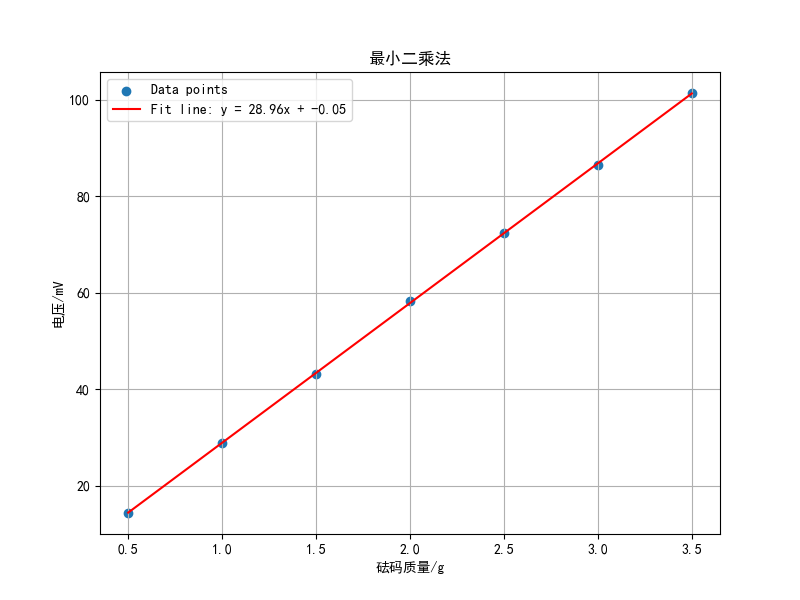
\includegraphics[width=0.8\textwidth,height=0.5\textwidth]{img/photo.png}
		%\caption{}
		\label{fig:side:b} 
    \end{figure}
\subsection{测定纯水的液体表面张力以及表面张力系数}
根据表3 中数据 $U_1$、$U_2$、$\Delta U$,带入公式
\begin{align*}
    F &= \frac{U_1-U_2}{k} = \frac{\Delta U}{k} \\
    \alpha &= \frac{F}{\pi(D_1+D_2)}
\end{align*}
其中 $(D_1+D_2) = 6.7956 \times 10^{-3} \ m$ 可得到纯水的液体表面张力及表面张力系数如下表

\hspace{-2cm}
\begin{table}[H]
\caption{纯水的液体表面张力系数的测量数据}
\begin{tabular}{|c|c|c|c|c|c|c|}
\hline
     测量次数 & 1 & 2 & 3 & 4 & 5  & 平均值 \\
\hline
     表面张力$F/N$ & 14.21 & 14.08 & 14.21 & 14.08 & 14.21  & 14.158 \\ 
\hline
     表面张力系数 $\alpha \  10^{-3}N/m$ & 66.56 & 65.95 & 66.56 & 65.95  & 66.56 & 66.31\\
\hline
\end{tabular}
\end{table}
其中在实验过程中的室温约为$22^{\circ}C$。纯水在$22^{\circ}C$条件下的标准液体表面张力系数为 $\alpha_{real} = 72.44 \times 10^{-3} N/m$

与标准值的绝对误差为 $\Delta \alpha = 72.44 - 66.31 N/m = 6.13 \times 10^{-3} N/m$

相对误差为  $E=\frac{\Delta \alpha}{\alpha_{real}}\times 100\% = 8.46\%$

\subsection{测定乙醇的液体表面张力和液体表面张力系数}
同$\S 3.2$ 中求纯水的表面张力和表面张力系数方法一致。结合表4中数据 $U_1$、$U_2$、$\Delta U$
可得到与表 类似的数据表格
\begin{table}
\caption{乙醇的液体表面张力系数的测量数据}
\begin{tabular}{|c|c|c|c|c|c|c|}
\hline
     测量次数 & 1 & 2 & 3 & 4 & 5  & 平均值 \\
\hline
     表面张力$F/N$ & 5.08 & 5.04 & 5.04 & 5.08& 5.04  & 5.056 \\ 
\hline
     表面张力系数 $\alpha \  10^{-3}N/m$ & 23.80& 23.61 &23.61 & 23.80&23.61  &23.68 \\
\hline
\end{tabular}
\end{table}

其中在实验过程中的室温约为$22^{\circ}C$。乙醇在$22^{\circ}C$条件下的标准液体表面张力系数为 $\alpha_{real} = 22.23 \times 10^{-3} N/m$

与标准值的误差为 $\Delta \alpha = 23.68 - 22.23 N/m = 1.45 \times 10^{-3} N/m$

相对误差为  $E=\frac{\Delta \alpha}{\alpha_{real}}\times 100\% = 6.52\%$
\section{结果讨论}
22$^{\circ}C$ 时纯水和乙醇的测定数据相对误差分别为$8.46\%$ 和 $6.52\%$ 。二者误差均偏大,可能是由于测量吊环时读数误差偏大,从而导致拟合系数$k$偏大,从而导致整体相对误差偏大;也有可能是水体遭到污染。

\section{思考题}
一.液体表面张力系数与液体的纯净度/杂质含量有关,与温度有关、与表面活性剂添加的剂量有关

二.常见测量方法有毛细管上升法、挂环法、威廉米平板法、旋转滴法、悬滴法等
\end{document}